\documentclass{standalone}
\usepackage{plotstyle}

\begin{document}

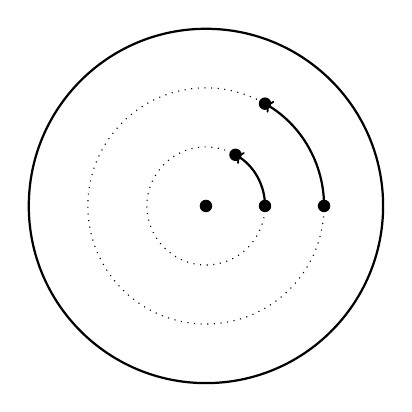
\begin{tikzpicture}[scale=0.75]
    % Define the center point and common angle
    \coordinate (O) at (0,0);
    \newcommand{\arcangle}{60} % Angle subtended by the arcs
    
        % Define radii and starting angles
    \foreach \r/\start in {1/0, 2/0} {
        % Draw each arc with an arrow
        \draw[thick, ->] 
            (\start:\r) arc[start angle=\start, end angle=\start+\arcangle, radius=\r];
                % Draw points at the start and end of each arc
        \fill[black] (\start:\r) circle (3pt); % Start point
        \fill[black] (\start+\arcangle:\r) circle (3pt); % End point
    }
    % Optional: Draw the center point
    \fill (O) circle (3pt) node[below right] {};
    \draw[thick] (O) circle (3);
    \draw[dotted] (O) circle (2);
    \draw[dotted] (O) circle (1);
    % \node at (\rtheta{2.3}{30}) {$s$};
\end{tikzpicture}
\end{document}